\section{Riemannsummen (Riemannintegral)}
\subsection{Riemansumme}
Wir betrachten die folgende Einteilung des Intervals $[a,b]$:\[
E: [a,b] = \bigcup_{k=1}^{N}[x_{k-1}, x_k] \text{ mit } x_k = a + k \cdot \frac{b-a}{N}.
\]
Die Feinheit dieser Zerlegung ist:\[
\delta(E) \equiv max\{x_k - x_{k-1}|k = 1...N\} = \frac{b-a}{N} \xrightarrow{N \to \infty} = 0
\]
$\xi_i$ sein ein Punkt auf dem Interval $[x_{i-1}, x_i]$, somit $\xi_i \in[x_{i-1}, x_i]$.\\

\begin{figure}
	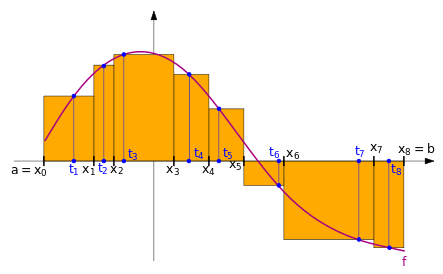
\includegraphics[width=\columnwidth]{riemann.png}
	\caption[Bildunterschrift]{Darstellung Riemannintegral mit $\xi_i = t_i$ und unsymetrischer Intervaleinteilung $E$.}
\end{figure}

Somit können wir die Riemannsumme bilden:
\begin{align*}
\int_a^b f(x)\;dx &=\sum (f,E,\xi)\\
&= \lim_{N \to \infty} \underbrace{\sum_{k=0}^{N-1}
\underbrace{f(\xi_i)}_{\text{``Höhe''}} \cdot
\underbrace{\delta(E)}_{\text{``Länge''}}}_{\text{Riemann-Summe}}\\
&= \lim_{N \to \infty} \sum_{k=0}^{N-1} {f(a +
k\frac{b-a}{N})} \cdot \frac{b-a}{N}
\end{align*}


\subsection{Riemann Integrabel}
Die Funktion $f$ sei Riemann Integrabel wenn es ein $I \in \R$ gibt so dass: $\forall \epsilon > 0, \exists \nu > 0$ so dass \[
|I| - \epsilon < \sum (f,E,\xi) < |I| + \epsilon
\]
für jede Einteilung $E$ von $[a,b]$ mit $\delta(E) < \nu$, und für jede Wahl von Zwischenpunkten $\xi$.\\
% Lamma aus http://www.mat.univie.ac.at/~kriegl/Skripten/math4ilak2/node18.html
Jede monotone Funktion und jede stetige Funktion ist Riemann-integrierbar.
\subsection{Beispiel}
Es soll das Intergral mittels Riemannschen Summe berechnet werden: $\int_a^b
e^{\lambda x}\,dx, \; \lambda \in \R$. $f(x) = e^{\lambda x}$

Zuerst unterteilt man das Intervall $[a,b]$: $E: [a,b] =
\bigcup_{k=1}^N[c_{k-1}, c_k]$ mit $c_k = a + k\cdot \frac{b-a}{N}$.

Die Feinheit dieser Zerlegung ist somit $\delta(E) = \max\{c_k - c_{k-1} | k =
1 \ldots N\} = \frac{b-a}{N}$. Dabei gilt $\delta(E) = \frac{b-a}{N} \to 0$ ($N
\to \infty$). Dies ist wichtig. Wir müssen die Feinheit unglaublich klein
bekommen können, also nahezu $0$. Je feiner die Feinheit desto genauer wird
unsere Riemann'sche Summe. Der Grenzwert dieser Summe für $N \to \infty$ ist der
Wert des bestimmten Riemann-Integrals.

Zusätzlich müssen wir festlegen, an welchen Punkten in den Teilintervallen wir
den Funktionswert auswerten. Hier legen wir fest: $x_k = c_{k-1}$, also
jeweils am Punkt an dem das Teilintervall beginnt.

Daraus erhalten wir nun:
\begin{align*}
\int_a^b e^{\lambda x}\;dx &= \lim_{N \to \infty} \underbrace{\sum_{k=0}^{N-1}
\underbrace{f(x_k)}_{\text{``Höhe''}} \cdot
\underbrace{\delta(E)}_{\text{``Länge''}}}_{\text{Riemann-Summe}}\\
&= \lim_{N \to \infty} \sum_{k=0}^{N-1} \underbrace{e^{\lambda (a +
k\frac{b-a}{N})}}_{f(x_k)} \underbrace{\frac{b-a}{N}}_{\delta(E)}\\
&= \lim_{N \to \infty} \frac{b-a}{N} e^{\lambda a} \sum_{k=0}^{N-1}(e^{\lambda
\frac{b-a}{N}})^k\\
&= \lim_{N \to \infty} \frac{b-a}{N} e^{\lambda a} \frac{1-e^{\lambda
(b-a)}}{1-e^{\lambda \frac{b-a}{N}}}
\end{align*}

Wir wissen, dass $\rho = \frac{b-a}{N} \to 0$ für $N \to \infty$. Somit
ersetzten wir es entsprechend:
\begin{align*}
\int_a^b e^{\lambda x}\;dx &= \lim_{\rho \to 0} \rho \cdot e^{\lambda a} \cdot
\frac{1-e^{\lambda(b-a)}}{1-e^{\lambda \rho}}\\
&= \lim_{\rho \to 0} \frac{\rho (e^{\lambda a} - e^{\lambda b})}{1-e^{\lambda
\rho}}\\
&\overset{\text{d'H}}= \lim_{\rho \to 0} \frac{e^{\lambda a} - e^{\lambda
b}}{-\lambda e^{\lambda \rho}}\\
&= \frac{e^{\lambda a} - e^{\lambda b}}{-\lambda} = \frac{1}{\lambda}(e^{\lambda
a} - e^{\lambda b})
\end{align*}
